
% 
% Annual Cognitive Science Conference
% Sample LaTeX Paper -- Proceedings Format
% 

% Original : Ashwin Ram (ashwin@cc.gatech.edu)       04/01/1994
% Modified : Johanna Moore (jmoore@cs.pitt.edu)      03/17/1995
% Modified : David Noelle (noelle@ucsd.edu)          03/15/1996
% Modified : Pat Langley (langley@cs.stanford.edu)   01/26/1997
% Latex2e corrections by Ramin Charles Nakisa        01/28/1997 
% Modified : Tina Eliassi-Rad (eliassi@cs.wisc.edu)  01/31/1998
% Modified : Trisha Yannuzzi (trisha@ircs.upenn.edu) 12/28/1999 (in process)
% Modified : Mary Ellen Foster (M.E.Foster@ed.ac.uk) 12/11/2000
% Modified : Ken Forbus                              01/23/2004
% Modified : Eli M. Silk (esilk@pitt.edu)            05/24/2005
% Modified : Niels Taatgen (taatgen@cmu.edu)         10/24/2006
% Modified : David Noelle (dnoelle@ucmerced.edu)     11/19/2014

%% Change ''letterpaper'' in the following line to ''a4paper'' if you must.

\documentclass[10pt,letterpaper]{article}

\usepackage{cogsci}
\usepackage{pslatex}
\usepackage{apacite}
\usepackage{amsmath,amssymb}
\usepackage{graphicx}
\usepackage{color}
\usepackage{url}
\usepackage{todonotes}
\usepackage{mathtools}
\usepackage{stmaryrd}
\usepackage{booktabs}

\newcommand{\den}[2][]{
\(
\left\llbracket\;\text{#2}\;\right\rrbracket^{#1}
\)
}

%\newcommand{\url}[1]{$#1$}

\definecolor{Blue}{RGB}{0,0,255}
\definecolor{Red}{RGB}{255,0,0}
\newcommand{\red}[1]{\textcolor{Red}{#1}}
\definecolor{Green}{RGB}{10,200,100}
\newcommand{\ndg}[1]{\textcolor{Green}{[ndg: #1]}}
\newcommand{\jd}[1]{\textcolor{Blue}{[jd: #1]}}  

 \newcommand{\denote}[1]{\mbox{ $[\![ #1 ]\!]$}}


\newcommand{\subsubsubsection}[1]{{\em #1}}
\newcommand{\eref}[1]{(\ref{#1})}
\newcommand{\tableref}[1]{Table \ref{#1}}
\newcommand{\figref}[1]{Figure \ref{#1}}
\newcommand{\appref}[1]{Appendix \ref{#1}}
\newcommand{\sectionref}[1]{Section \ref{#1}}

\title{Animal, dog, or dalmatian? Level of abstraction in nominal referring expressions}
%Animal, dog, or dalmatian? Contextual informativeness, utterance length and utterance frequency affect choice of referring expressions.

 
\author{{\large \bf Caroline Graf, Judith Degen, Robert Hawkins, Noah D.~Goodman} \\
  cgraf@uos.de, \{jdegen,rxdh,ngoodman\}@stanford.edu\\
  Department of Psychology, 450 Serra Mall \\
  Stanford, CA 94305 USA}



\begin{document}

\maketitle


\begin{abstract}

\red{The choice of referring expressions is highly context dependent. Whether speakers choose to refer to an object as a ``dalmatian'', a ``dog'', or an ``animal'' is determined partly by the features of the other objects present in the scene, as well as features of the utterance alternatives. The current study within a reference game setting demonstrates that speakers' choice of referring expression is dependent on a rich interplay of the expression's degree of contextual informativeness, its relative length and its relative frequency. If a competitor object of the same category (e.g., dog) as the target object is present in the display, speakers choose a more specific subcategory (e.g., ``dalmatian'') to refer to the target object. In contrast, when the competitor objects do not share the same (super-) category as the target, speakers are less constrained in choosing an appropriate referring expression. In this event, shorter expressions are preferred over longer ones and more frequent category names are preferred over less frequent ones. The pattern of results is predicted by a production model couched in the Rational Speech Act framework, in which a speaker is modeled as balancing an utterance's contextual informativeness with its cost relative to its alternatives.}

\textbf{Keywords:} 
referential expressions, levels of reference, overinformativeness, basic levels, categorization
\end{abstract}

\section{\bf Introduction}

\todo[inline]{rdh: can we begin by setting up the puzzle of basic-level reference, and \emph{then} set up connections with overinformativity, rational models, etc.? (e.g. ``There are many ways to refer to any given object. If you see a man walking a dalmatian down the street, you could tell your friend about it using ``dalmatian,'' ``dog,'' ``animal,'' or even ``living thing'' and all would be true. By the age of three, children are willing to accept multiple labels for the same object, at different levels of abstraction \cite{WaxmanHatch92_BasicLevelLabeling}. How do speakers manage this broad flexibility in the choice of referring expression?)}
One of the main purposes of language is communication. In fact, some cognitive scientists have gone as far as proposing that language may simply be a special case of social cognition: Speakers choose an utterance approximately optimally such that a listener can infer the intended meaning by means of Bayesian inference \cite{frank2012}. According to this view, language is essentially about reasoning about other people's knowledge, states and intentions. An important assumption here is that the speaker is a rational agent, who selects an utterance based on its optimal expected utility. 

Although approaches in this framework have been increasingly successful in predicting human behavior, past research in the area of referential expressions has demonstrated that speakers are not necessarily behaving in a rational manner when it comes to producing referential expressions. For instance when subjects tend to overly produce color modifiers to describe objects, even if color is not an attribute necessary for disambiguation (e.g. Pechmann, 1989; Sedivy, 2003). For example, when subjects are being shown a small red cup as a target object in the context of a big red cup and a big blue cup and asked to describe the target, a significant amount of subjects say ``small red cup'', when ``small cup'' would have been sufficient for disambiguation. Speakers are producing overinformative utterances and can thus be said to be irrational in their behavior (Gatt et al., 2012). 

\todo[inline]{rdh: I spruced up this paragraph about Rosch and the basic-level literature!}
In a series of classic experiments on the structure of concepts, Eleanor Rosch and colleagues established that there is a maximally informative level of abstraction in category taxonomies. Dogs have a large number of features in common -- four legs, wagging tail, loyal companion -- which differentiate them from other animals, but there are fewer features that distinguish dalmatians from german shepherds. She called this level of abstraction (e.g. ``dog'') the \emph{basic level} \cite{RoschEtAl76_BasicLevel}. Among other consequences of this structure, participants in a free-response naming task were much more likely to use the basic-level than the superordinate level of subordinate level, even though they knew all three terms. Subsequent studies showed that the preferred level of reference depends on expertise \cite{TanakaTaylor91_BasicLevelAndExpertise} and context \cite{JohnHampsonGoldbert91_BasicLevelPersonality}.

\todo[inline]{rdh: Wherever we end up putting the previous paragraph, it might be nice to follow it with a paragraph suggesting that we should also expect basic-level reference to be affected by communicative pressures}

%Seen in the light of overinformativeness, one might argue that speakers act in an overinformative manner when describing an object in a more specific way than is necessary for disambiguation, for example when saying ``dog'' in the above scenario instead of calling the object an ``animal''. But under what circumstances do speakers actually use the basic level and when do they revert to the sub- or superlevel? Which other factors contribute to the choice of utterance and is there a way to manipulate the speaker's behavior? 

Including more attributes than are necessary to identify a target object may at first seem to contradict the Maxim of Quantity by Grice (1975), namely to make one's contribution as informative than is required and not more, but what does it actually mean for an utterance to be more informative than *required*? Does it mean that this utterance mentions attributes redundantly irrespective of their utility? What if the so called ``redundant'' attributes (e.g. Arts, 2004; Arts, Maes, Jansen, \& Noordman, 2011) actually have an utility after all by influencing the processing of an utterance? Pechmann (1985) has argued that the excessive use of color adjectives in referential expressions does in fact contribute to the informativeness of the utterance, namely by excluding some (but not all) distractors. As a matter of fact, other studies have demonstrated that overspecified utterances give rise to shorter identification times compared to minimally specified expressions (Deutsch, 1976; Sonnenschein, 1982). Thus, ``overinformative'' behavior must not necessarily be irrational behavior. 

A similar argument can be made for the the use of a level of reference less abstract than necessary for disambiguation and the dominance for the the basic level in the production of referential expressions. The basic level of reference, which Rosch et. al (1976) characterize as the level of abstraction at which the most basic category cuts are made, seems to have a special status in human categorization behavior: Basic level categoriy labels are not only the first labels used for categorization during perception of the environment, but also the labels which lead to fastest category verification. Basic levels also carry the most information and possess the highest category cue validity (compared with the sublevel ``dalmatian'' or superlevel ``animal''). Therefore it can be argued that being more specific than necessary has a positive effect on the processing of the utterance for the listener and thus ``overinformativeness'' contributes to the informativeness of the utterance.

The following experiment explores what effect context has on the choice of referring expression by varying the level of reference of the distractor objects; distractors may be from the same basic level category or the same super level category as the target object or belong to neither. Furthermore we investigate whether and under what circumstances the basic level is preferred, how important of a role informativeness plays and what specific aspects of the labels, particularly length and frequency, are other factors contributing to the selection of utterance. 

\section{\bf Methods}

\ndg{i think we want procedure and design figure(s). the procedure fig should show a screen shot from speaker and listener points of view. the design fig should illustrate the dist12, etc notation used later with a concrete domain.}

\subsection{\bf Participants}
We recruited 56 participants over Amazon's Mechanical Turk who were self-reported native speakers of English. Participants completed the experiment in pairs of two.

\subsection{\bf Materials}
Stimuli were selected from eight distinct domains. These domains represented basic level categories such as ``dog'', for each of which four target images were chosen, corresponding to four subcategories of this domain (e.g. ``dalmatian'', ``pug'', ``German Shepherd'' and ``husky''). Each domain also contained an additional item which belonged to the same basic level category as the targets (e.g. ``greyhound'') as well as items which belonged to the same supercategory but not the same basic level (e.g. ``elephant'' or ``squirrel''). 

\subsection{\bf Design}
Each trial consisted of a display of three pictures of objects, one of which was designated as the target object. There were four target objects for each of the eight domains, each of which would appear once for every pair, giving rise to a total of 36 trials per pair. There were four conditions which differed in the types of distractors which were shown: (a) {\bf distractor12}: one distractor of the same basic level and one distractor of the same superlevel were present (e.g. target: ``dalmatian'', distractor 1: ``greyhound'', distractor 2: ``squirrel''), (b) {\bf distractor22}: two distractors of the same superlevel were present, (c) {\bf distractor23}: one distractor of the same superlevel and one artifact were present and (d) {\bf distractor33}: two artifacts were present. The selection of distractors was random for each trial. Furthermore, the experiment contained 36 filler items, in which participants were also asked to produce referential expressions for objects, but here the three pictures illustrated the same stimulus which differed only in size and color. No filler items were reused in the target trials.

\subsection{\bf Procedure}
Pairs of participants were connected through a real-time multi-player interface \cite{Hawkins15_RealTimeWebExperiments}. Subjects participated in pairs, with one member of each pair assigned the speaker role and the other to the listener role. Participants kept their allotted roles for the entire experiment. 
Each saw the same set of three images, however participants were informed that image placement would be (and in fact was) different for the speaker and the listener. The target object was identified by a green square surrounding it for the speaker (but not listener). There was a chatbox in which speaker and listener could send text messages to each other. The task was for the speaker to tell the listener which one of the objects is the target, and for the listener in turn to select the right object based on the information provided by the speaker. 

\subsection{\bf Annotation}
Responses were processed automatically to determine the level of reference used and subsequently checked manually for typos or meaning-equivalent alternatives (e.g., ``grizzly'' was counted as an instance of ``grizzly bear''). 
%\ndg{need to describe this parsing / coding in more detail.}
Trials on which the listener selected the wrong referent were excluded from the analysis, which led to the elimination of 1.1\% of trials. A further 10\% of trials were excluded because  the produced utterance named an attribute of the object rather than its type (e.g. ``can fly'' instead of ``bird'').

\section{\bf Results}

Proportions of sub, basic, and super level utterance choices in the different conditions are shown in \figref{fig:results1}. The sub level term was preferred where it was necessary for unambiguous referent identification, i.e., when a distractor of the same basic level category as the target was present in the scene (condition distr12, e.g., target: dalmatian, distractor: greyhound). Where it was not necessary (i.e., when there was no other object of the same basic level category present, as in conditions distr22, distr23 and distr33), there was a clear preference for the basic level term. The super level term was strongly dispreferred overall, though it was used on some trials, especially where informativeness constraints on utterance choice were weakest (condition distr33). 

\begin{figure}[ht!]
\centering
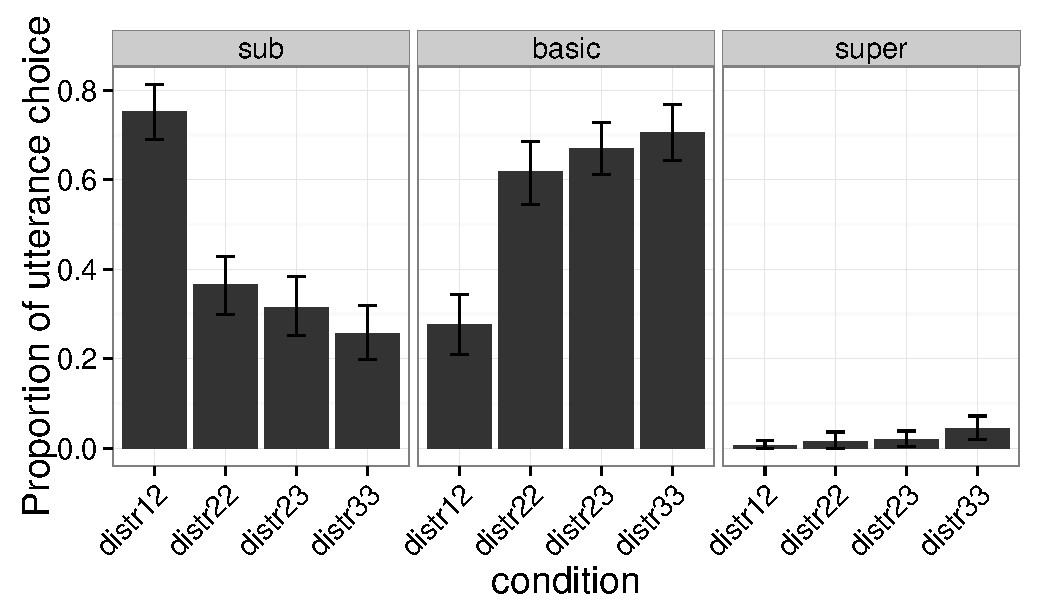
\includegraphics[width=.5\textwidth]{graphs/results-collapsed}
\caption{Proportion of utterance choice by condition. Error bars indicate bootstrapped 95\% confidence intervals.}
\label{fig:results1}
\end{figure}

To test for the independent effects of informativeness, length, and frequency on sub level mention, we conducted a mixed effects logistic regression. Frequency was coded as the difference between the sub and the basic level's log probability. Length was coded as the ratio of the sub to the basic level's length in characters. That is, a higher frequency difference indicates a \emph{lower} cost for the sub level term compared to the basic level, while a higher length ratio reflects a \emph{higher} cost for the sub level term compared to the basic level. Condition was coded as a three-level factor: \emph{sub necessary}, \emph{basic sufficient}, and \emph{super sufficient}, where distr22 and distr23 were collapsed into \emph{basic sufficient}. Condition was Helmert-coded: two contrasts over the three condition levels were included in the model, comparing each level against the mean of the remaining levels (in order: \emph{sub necessary}, \emph{basic sufficient}, \emph{super sufficient}). This allowed us to determine whether the probability of type mention  for neighboring conditions suggested by \figref{fig:results1} were significantly different from each other.\footnote{Adding terms that code the ratio of the sub vs super level frequency and length did not lead to an improvement of model fit.} The model included random by-speaker and by-domain intercepts. 



A model summary is shown in \tableref{tab:modelresults}. The log odds of mentioning the sub level term was greater in the \emph{sub necessary} condition than in either of the other two conditions, and greater in the \emph{basic sufficient} condition than in the \emph{super sufficient} condition, suggesting that the contextual informativeness of the sub level mention has a gradient effect on utterance choice. In addition, there was a main effect of length, such that as the length of the sub level term increased compared to the basic level term (``chihuahua''/``dog'' vs.~``pug''/``dog''), the sub level term was dispreferred (i.e., ``chihuahua'' is dispreferred compared to ``pug'', see \figref{fig:lengtheffect}). Finally, while there was no main effect of frequency, we observed a significant length by frequency interaction (visualized in \figref{fig:lengthfreqinteraction}), such that the length effect was greater for cases where sub level frequency compared to the basic level was relatively high. 


\begin{table}[!tbp]
\caption{Mixed effects model summary.}
\begin{center}
\begin{tabular}{lrrl}
\toprule
\multicolumn{1}{l}{}&\multicolumn{1}{c}{Coef $\beta$}&\multicolumn{1}{c}{SE($\beta$)}&\multicolumn{1}{c}{$p$}\tabularnewline
\midrule
Intercept&$-0.38$&$0.38$&\textgreater0.31\tabularnewline
Condition sub.vs.rest&$ 2.37$&$0.24$&\textbf{\textless.0001}\tabularnewline
Condition basic.vs.super&$ 0.53$&$0.22$&\textbf{\textless.05}\tabularnewline
Length&$-0.39$&$0.14$&\textbf{\textless.01}\tabularnewline
Frequency&$-0.09$&$0.06$&\textgreater0.17\tabularnewline
Length:Frequency&$-0.34$&$0.08$&\textbf{\textless.0001}\tabularnewline
\bottomrule
\end{tabular}\end{center}
\label{tab:modelresults}
\end{table}


\begin{figure}[ht!]
\centering
%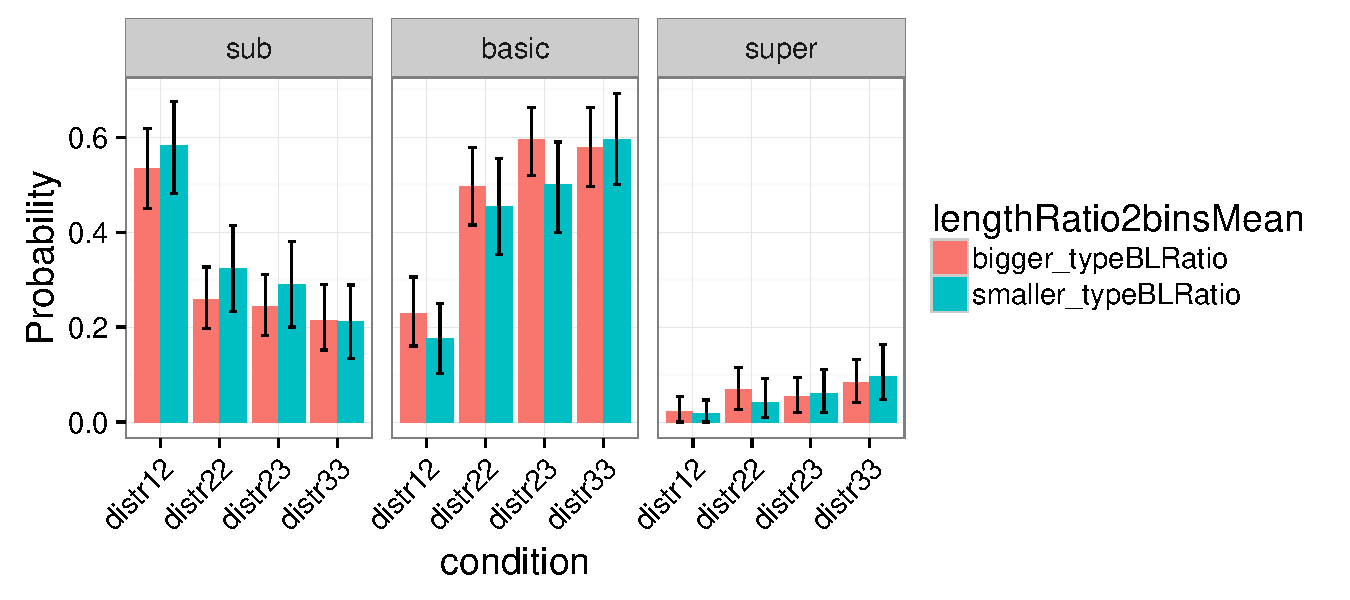
\includegraphics[width=.5\textwidth]{graphs/lengthRatio}
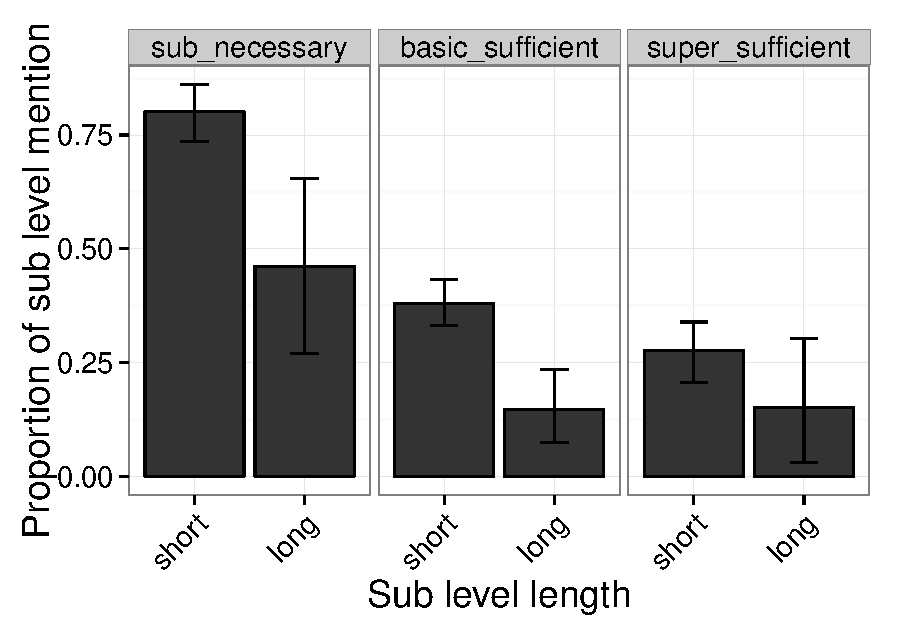
\includegraphics[width=.5\textwidth]{graphs/length-effect}
\caption{Probability of using sub, basic and super level terms when the sub  length is relatively short (.667,2] or long [2,4.67) compared to the basic level term length.}
 \label{fig:lengtheffect}
\end{figure}



\begin{figure}[ht!]
\centering
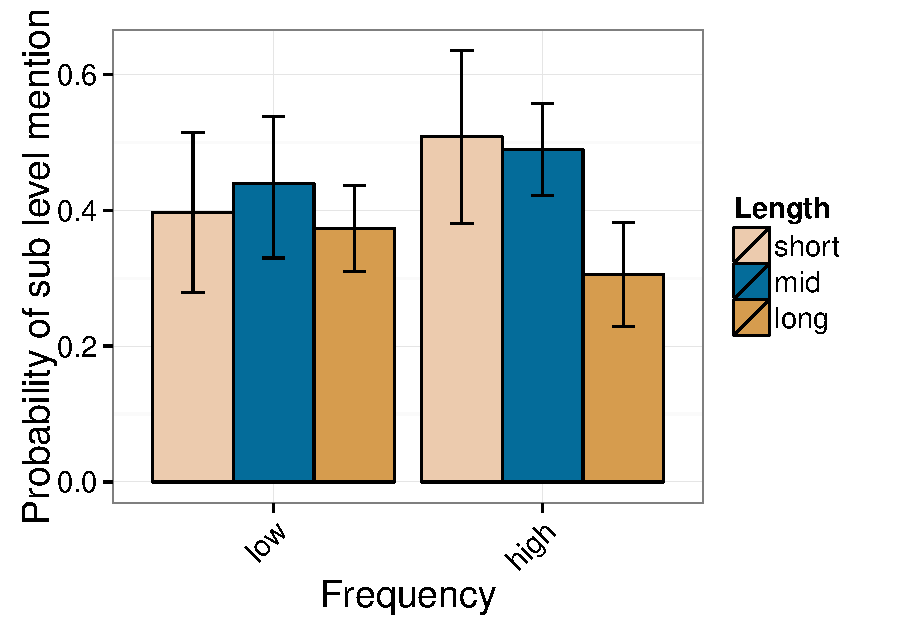
\includegraphics[width=.5\textwidth]{graphs/freq-length-interaction}
\caption{Proportion of sub level mentions  as a function of the sub level term's relative length and frequency compared to the basic level. Length bins reflect the sub/basic length ratio intervals (0, 1] (short), (1, 2] (mid), (2, 4.67] (long). Frequency bins reflect the sub/basic log frequency difference intervals (-11.2,-5.19] (low), (-5.19,-0.65] (high).}
\label{fig:lengthfreqinteraction}
\end{figure}


Unsurprisingly, there was also significant by-participant and by-domain variation in the log odds of sub level mention. \figref{fig:domains} shows the by-domain variation in utterance choice. For instance, mentioning the subclass over the basic level term was preferred more in some domains (e.g. in the ``candy'' domain) than in others. Likewise, some domains had a greater preference for basic level terms (e.g. the ``shirt'' domain). Using the superclass term also ranged from hardly being observable (e.g. the ``flower'' domain) to being used more frequently (e.g. in the ``bird'' domain). Nevertheless, mentioning the sublevel category was always the most frequent choice of utterance in the case where a distractor of the same basic level was displayed. Furthermore, the sublevel term was always mentioned most frequently and the basic level least frequently in just this condition, compared to the other three conditions.


\begin{figure}[ht!]
\centering
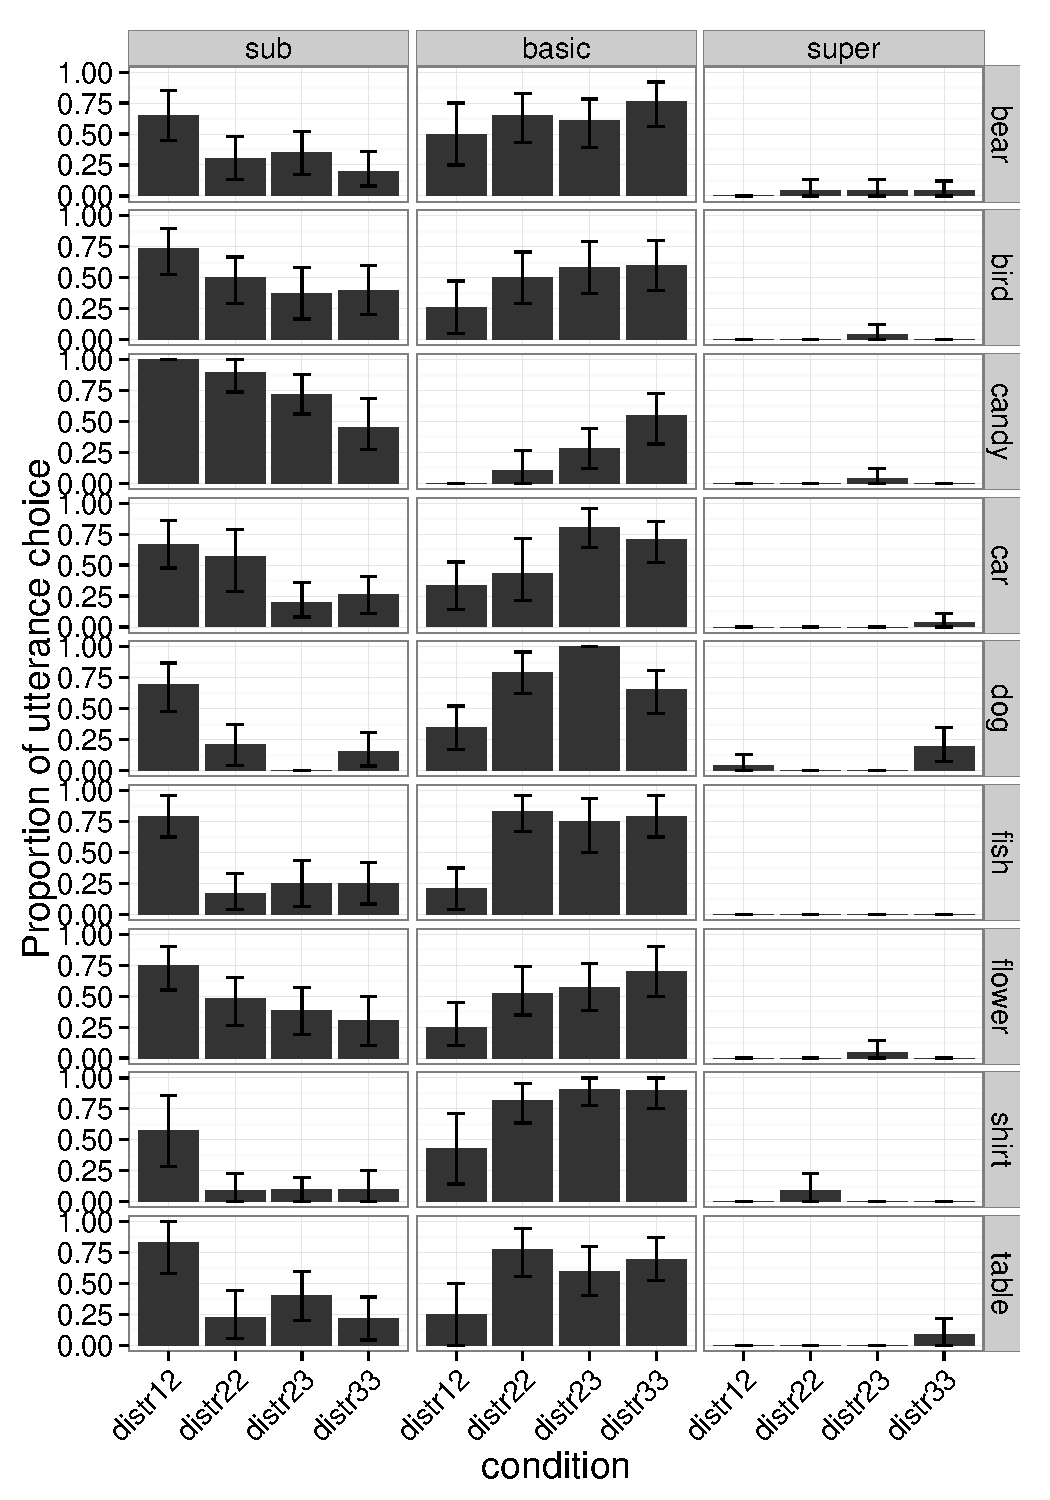
\includegraphics[width=.5\textwidth]{graphs/results-bydomain}
\caption{Proportion of utterance choice by domain and condition. Error bars indicate bootstrapped 95\% confidence intervals.}
\label{fig:domains}
\end{figure}

These results suggest that the choice of level of reference depends in a gradient manner on both the informativeness of the reference level as well as on the cost of the corresponding utterance (both in terms of length and frequency) compared to the alternative utterances.




\section{\bf Modeling level of reference}

To show that we can account for these context effects purely through communicative pressures, we formulated a simple probabilistic model of basic-level reference. As in earlier Rational Speech Act (RSA) models \cite{frank2012, goodmanstuhlmueller2013}, the speaker seeks to be informative with respect to an internal model of a literal listener, but also seeks to be parsimonious. The literal listener updates their beliefs to rule out possible worlds that are inconsistent with the meaning of the speaker's utterance. We incorporate length and frequency as costs that affect the speaker's likelihood of using a label, and we account for typicality as part of a label's graded meaning: the label ``dog'' fits a dalmatian better than a grizzly bear, but it also fits a grizzly bear better than a tennis ball.
\ndg{how we write this section depends partly on how important confusability (ie typicality) is to our story and whether we have item-wise data to plug in.}

Formally, we start by specifying a literal listener $L_0$ who hears a label $l$ in the context of some set of objects $\mathcal{O}$ and returns a response distribution over objects $o_i \in \mathcal{O}$ : 
$$P_{L_0}(o_i | l) \propto \denote{l}(o_i)$$
where $\denote{l}(o_i)$ is the lexical meaning of the label $l$ when applied to object $o_i$. We take this to be a real number indicating the degree of acceptability or typicality of object $o_i$ for category $l$. \ndg{adjust...}

Next, we specify a speaker $S_1$ who is attempting to refer to a particular object $o \in \mathcal{O}$ and chooses among possible labels $l_j \in \ell(o)$: 
$$P_{S_1}(l_j | o) \propto \exp\{\alpha \left( \ln P_{L_0}(o | l_j) + U_{cost}(l_j) \right) \}$$
where $U_{cost}(l_j)$ is the label cost function and $\alpha$ is an optimality parameter\footnote{$\alpha = 1$ corresponds to a soft-max decision rule, and $\alpha \rightarrow \infty$ corresponds to a optimal hard-max decision rule.}. \ndg{is there a parameter for relative importance of informativity and cost?}

Finally, we must specify the the lexical meaning function $\denote{l}(o_i)$ and the cost function $U_{cost}(l_j)$. 
\red{rdh: we'll probably want to write down how we compute length and frequency earlier, since some results depend on them.}
We measure label cost as the linear combination of two components: length and frequency. Length cost $c_l$ is defined as the number of characters in the label, and frequency cost $c_f$ is estimated using the log probability of occurring in the Google Books corpus from 1960 to the present. To trade these two measures off against one another, we compute normalized scores $\hat{c}_l \in [0,1]$ and $\hat{c}_f \in [0,1]$ by subtracting the minimum score of all labels used in the experiments and dividing by the range. We then define the label cost of $l_j$ to be $$U_{cost}(l_j) = w\hat{c}_f - (1-w)\hat{c}_l$$ where $w \in [0,1]$ is a parameter controlling the tradeoff between length and frequency.


\ndg{MODEL RESULTS AND ANALYSIS!!}


\section{\bf Discussion and conclusion}

\section{\bf Acknowledgments}

This work was supported by ONR grant N00014-13-1-0788 and a James S. McDonnell Foundation Scholar Award to NDG and an SNF Early Postdoc.Mobility Award to JD. RXDH was supported by the Stanford Graduate Fellowship and the National Science Foundation Graduate Research Fellowship under Grant No. DGE-114747.

\small


\bibliographystyle{apacite}

\setlength{\bibleftmargin}{.125in}
\setlength{\bibindent}{-\bibleftmargin}

\bibliography{bibs}


\end{document}
